\documentclass[a4paper,jou]{apa6}  % maakt het hele document op als een 'printed APA journal'.
\usepackage[utf8]{inputenc} % lettertype
\usepackage{authblk}
\usepackage[dutch]{babel} % afbreken van nederlandse woorden
\usepackage{enumitem} % genummerde lijsten toevoegen
\usepackage{apacite} % APA_style citaten
\usepackage{graphicx} % afbeeldingen toevoegen
\usepackage{amsfonts, amsmath, amsthm, amssymb} % voor wiskundesymbolen
\usepackage{wrapfig} % voor tekst rondom afbeeldingen
\usepackage{mdframed} % voor de lijnbox rondom de definities

\title{Bewustzijn heeft aandacht nodig: gistperceptie onder dualtaskcondities}
\shorttitle{Bewustzijn heeft aandacht nodig}
\author{Raoul Grouls, Libby van den Besselaar, Eva Bakels, Kiki von Piekartz}
\affiliation{Universiteit Utrecht}
\abstract{Bewustzijn zonder aandacht, is dat mogelijk? In dit onderzoek wordt dat onderzocht met behulp van het dualtask-paradigma. De participanten (n=34) moeten tegelijkertijd een aandachtstaak (bewegende objecten tellen) en een bewustzijnstaak (gistwaarneming) uitvoeren. Analyse van onze data toont aan (p=0.017) dat de gistwaarneming afneemt, naarmate de intensiteit van de aandachtstaak toeneemt. Dit impliceert dat bewustzijn aandacht nodig heeft, hoewel het niet is vast te stellen of bewustzijn onmogelijk is zonder aandacht.
}
\begin{document}
\maketitle
\begin{mdframed}
\small
\textbf{Aandacht} Topdown, selectieve aandacht. Door selectieve aandacht wordt informatie diepgaander verwerkt \cite{Cohen_Cavanagh_Chun_Nakayama_2012}. Topdown betekent aandacht die bewust wordt gestuurd.\\ 
\textbf{Bewustzijn} Inhouden van het bewustzijn; expliciet geen niveaus van bewustzijn zoals waken of slapen \cite{VanBoxtel_Tsuchiya_Koch_2010}.\\
\textbf{Gistwaarneming} Indruk van de getoonde scene in hoofdlijnen  die achterblijft na het zeer kort (30ms) vertonen van een afbeelding \cite{Mack_Clarke_2012}.\\
\textbf{Dual-task paradigma} Hierbij moet de proefpersoon twee taken tegelijk uitvoeren, zodat de mogelijke interferentie tussen de twee typen taken kan worden blootgelegd \cite{Reddy_Reddy_Koch_2006}\\
\textbf{Flash supression} Het tijdelijk onderdrukken van het bewustzijn van een getoonde afbeelding aan \'e\'en oog, wanneer tegelijkertijd aan het andere oog snel wisselende random patronen getoond worden. \cite{Sklar_Levy_Goldstein_Mandel_Maril_Hassin_2012}
\end{mdframed}

\section*{Introductie}
\subsection{Twee stromingen} 
Kan het een bestaan zonder het ander? De discussie over de relatie tussen aandacht en bewustzijn wordt gedomineerd door ruwweg twee standpunten. De eerste stroming stelt dat bewustzijn en aandacht los van elkaar kunnen bestaan \cite{Block_2011}. Daartegenover staat de stroming die stelt dat bewustzijn en aandacht onlosmakelijk met elkaar verbonden zijn \cite{Cohen_Dennett_2011}. Deze stellingname wordt in later onderzoek afgezwakt naar de stelling dat met name bewustzijn niet kan bestaan zonder aandacht \cite{Cohen_Cavanagh_Chun_Nakayama_2012}. 
\subsubsection{Aandacht zonder bewustzijn}
Verschillende onderzoeken bewijzen dat aandacht zonder bewustzijn bestaat. Zo kunnen via de techniek van flash suppression teksten of afbeeldingen worden getoond, zonder dat mensen zich bewust worden van die tekst of afbeelding. Mensen blijken echter wel degelijk de inhoud van het getoonde te verwerken. Zo is aangetoond dat mensen, zonder daar bewust van te zijn, rekensommen of de semantiek van taal kunnen verwerken \cite{Sklar_Levy_Goldstein_Mandel_Maril_Hassin_2012}. Proefpersonen werden zich sneller bewust van gramaticaal onjuiste zinnen dan van juiste zinnen, wanneer zij deze getoond kregen via flash suppression. Verder kiezen zij eerder de juiste uitkomst van een onbewust waargenomen rekensom. Ook is aangetoond dat de ruimtelijke aandacht van proefpersonen wordt getrokken naar een erotische afbeelding, afhankelijk van hun seksuele oriëntatie, ondanks dat deze via flash suppression onzichtbaar werden gemaakt \cite{Jiang_Costello_Fang_Huang_He_2006}. Op basis van deze en andere vergelijkbare onderzoeken concluderen zelfs prominente voorstander van de onscheidbaarheid van aandacht en bewustzijn dat aandacht zonder bewustzijn inderdaad bestaat:“aandacht kan ingezet en gestuurd worden richting stimuli die niet bewust zijn waargenomen”\cite{Cohen_Cavanagh_Chun_Nakayama_2012}.
\subsubsection{Bewustzijn zonder aandacht}
De discussie tussen de twee stromingen spitst zich door deze conclusie van Cohen et al. (2012) toe op de vraag of bewustzijn zonder aandacht mogelijk is. Dit artikel zich daarom verder op deze laatste vraagstelling.
Door zowel voor- als tegenstanders van deze stelling wordt onderzoek naar gistwaarneming onder een dualtask paradigma geaccepteerd als acceptabele manier om dit vraagstuk te onderzoeken \cite{Block_2011,Cohen_Cavanagh_Chun_Nakayama_2012}. Er zijn diverse onderzoeken die aantonen dat gistwaarneming inderdaad mogelijk is onder dual-task condities \cite{LiVanRullenKochPerona2002,Reddy_Reddy_Koch_2006,VanBoxtel_Tsuchiya_Koch_2010,oliva2006building}, onder andere voor het bepalen van gender, de identiteit van bekende personen en natuurscenes. Er wordt hierbij uitgegaan dat er een beperkte capaciteit van aandacht te verdelen is. Wanneer deze beperkte capaciteit in voldoende mate gemonopoliseerd is, kan deze niet meer beschikbaar zijn voor de gistwaarneming en is dus het feit dat de gistwaarneming alsnog plaatsvindt bewijs voor het onafhankelijk zijn van bewustzijn voor aandacht \cite{Mack_Clarke_2012,Cohen_Cavanagh_Chun_Nakayama_2012}. 
\subsection{Kritiek- en verbeterpunten}
\subsubsection{Mogelijke spill-over van aandacht} Dit is meteen het zwakke punt van de onderzoeken die tot nu toe gedaan zijn: het is niet definitief uit te sluiten dat werkelijk alle aandacht wordt gemonopoliseerd. Diverse artikelen die gist onderzoeken nemen dan ook in hun titel een zinsnede op als \textquotedblright in the near-absence of attention\textquotedblleft\; \cite{LiVanRullenKochPerona2002,Reddy_Reddy_Koch_2006}. Cohen et al. (2012) wijzen op een mogelijke \textquotedblright spill over\textquotedblleft\;van aandacht: als de aandachtstaak niet veeleisend genoeg is, zou er nog een beetje van de aandacht gebruikt kunnen worden voor de gistwaarneming. Zij hebben daarom onderzoek opgezet waarbij de aandachtstaak zeer veeleisend is gemaakt \cite{Mack_Clarke_2012,Cohen_Cavanagh_Chun_Nakayama_2012}. Zij gebruiken daarbij technieken om de aandachtstaak veeleisender te maken en zo de spill over van aandacht te verkleinen zoals masking (na de stimulus vult het beeld zich met patronen). De onafhankelijke variabele in deze onderzoeken is de aandachtinstructie. Er bestaat een eerste conditie waarbij geen instructie wordt gegeven; een tweede conditie waarbij wordt verteld dat er iets in beeld verschijnt maar de focus bij de aandachtstaak moeten blijven; een derde conditie waarbij de proefpersoon de aandachtstaak mag loslaten om te speuren naar iets wat mogelijk in beeld verschijnt. Er wordt onder deze condities gevonden dat de groep met de instructie om de aandachtstaak los te laten, beter in staat is om de gist waar te nemen dan wanneer de proefpersonen in het ongewisse worden gelaten \cite{Mack_Clarke_2012,Cohen_Cavanagh_Chun_Nakayama_2012}.
\subsubsection{Beperkingen van de aandachtsinstructie}
Deze onderzoeksopzet heeft echter een aantal mankement. Door technieken zoals masking te combineren met een aandachtsinstructie als onafhankelijke variabele, bestaat het risico dat we de biologische beperkingen van het oog meten, in plaats van het monopoliseren van aandacht. Er worden namelijk naast de aandachtsinstructie ook oogbewegingen ge\"introduceerd, die als contaminerende variabele kunnen optreden. Proefpersonen kunnen in de periferie namelijk minder detail waarnemen, dan in het centrum van de focus \cite{moore2013clinically}. Dit kan voorkomen worden door de aandachtsinstructie constant te houden en als onafhankelijke variabele de intensiteit van de aandachtstaak te vari\"eren.
\subsubsection{Intensiteit als onafhankelijke variabele}
In ons onderzoek sluiten we daarom aan op de door anderen gebruikte globale opzet met een centrale aandachtstaak en perifere gistwaarneming onder dual-task condities. Als onafhankelijke variabele is, in tegenstelling tot het onderzoek van Mack \& Clarke (2012), gekozen voor een aandachtstaak die varieert in intensiteit. Hiermee wordt evenmin uitgesloten dat er een residu van aandacht overblijft, maar het is aannemelijk dat een eventuele interferentie tussen aandacht en bewustzijn op deze manier zichtbaar wordt.
De opzet van Alvarez en Oliva (2008) met een \textit{multiple-object tracking task} is gebruikt als basis voor een veeleisende aandachtstaak. Bij deze taak moesten proefpersonen diverse bewegende objecten volgen. Het voordeel van dit type aandachtstaak is dat de hoeveelheid vereiste aandacht gemakkelijk aan te vari\"eren is. Met vier objecten wordt er meer aandacht gevraagt dan met twee objecten, zonder dat de test verder al te veel wordt aangepast. 
\subsubsection{Hypothese}
Wanneer de aandachtstaak in intensiteit toeneemt, zal de beschikbare aandacht in toenemende mate worden gemonopoliseerd voor deze taak. Indien aandacht een voorwaarde is voor bewustzijn zal het percentage correcte gistwaarnemingen afnemen. Wanneer aandacht geen voorwaarde is voor bewustzijn, zullen beide taken niet interfereren en zal het percentage gistwaarnemingen niet afnemen bij een toenemende intensiteit van de aandachtstaak. Wij hypothetiseren het volgende (zie fig. \ref{fig:hypothese}):
\begin{quote}
\textit{Als we de intensiteit van aandachtstaak $x$ noemen het de gistwaarneming $y$ noemen, kunnen we de relatie tussen beide modelleren volgens $f(y)=ax+b$. Wanneer aandacht een voorwaarde is voor bewustzijn, zal voor de waarde van $a$ gelden dat $a<0$. Wanneer aandacht geen voorwaarde is voor bewustzijn, zal voor de waarde van $a$ gelden dat $a=0$}
\end{quote}
\begin{figure}
\centering
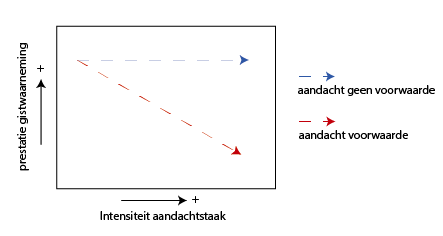
\includegraphics[width=1.0\linewidth]{illustratieHypothese.png}
\caption{\label{fig:hypothese}De visualisatie van onze hypothese.}
\end{figure}
\section*{Methode}
\subsection{Participanten} 
Bij het selecteren van proefpersonen voor dit onderzoek is gestreefd naar een evenwichtige spreiding van leeftijd (zie tabel \ref{tab:leeftijden}).
% ik volg deze opmaak https://owl.english.purdue.edu/owl/resource/560/19/
\begin{table}
\caption{\label{tab:leeftijden}Spreiding leeftijden}
\begin{tabular}{c c c c c c c}
\hline
	& \underline{median} & \underline{mean} & \underline{sd} & \underline{min} & \underline{max} & \underline{n}\\
	totaal & 22 & 30.5 & 15.2 & 17 & 60 & 34\\
	vrouwen & 20 & 24.0 & 11.0 & 17 & 55 & 17\\
	mannen & 39 & 37.1 & 16.3 & 18 & 60 & 17\\
\hline
\end{tabular}
\end{table}
Bij de selectie van participanten voor dit onderzoek is rekening gehouden met de etniciteit van proefpersonen, omdat verwacht werd dat dit mogelijk invloed zou kunnen hebben op het herkennen van de gezichten\cite{sporer2001recognizing}.
\subsection{Materiaal}
Het experiment is opgezet met behulp van PsychoPy2 software \cite{peirce2007psychopy, Peirce2009generating}. Dit is opensource-software, bedoeld voor neuroscience onderzoek en gebaseerd op de programmeertaal Python. PsychoPy2 geeft de ruimte om het experiment met eigen pythoncode aan te passen, waar we vooral gebruik van hebben gemaakt voor het randomiseren van de stimuli. Het PsychoPy-experiment werd geïnstalleerd op diverse MacBook-Pro-laptops (2011-2013) op een resolutie van 1280x800, waarmee de proefpersonen de test maken. De resultaten zijn geanalyseerd met het R-softwarepakket \cite{Rsoftware}. De complete code inclusief de gebruikte fotos zijn te vinden op GitHub \cite{Grouls2017}.
\subsection{Stimuli} Op een grijs scherm verschenen gedurende 6.0s steeds 2 tot 4 ronde, blauwe objecten (zie figuur \ref{fig:tijdlijnExperiment}). Deze objecten waren 5 pixels groot en volgden in zowel de x- als de y-richting een sinusgolf. 
\begin{figure}
\centering
	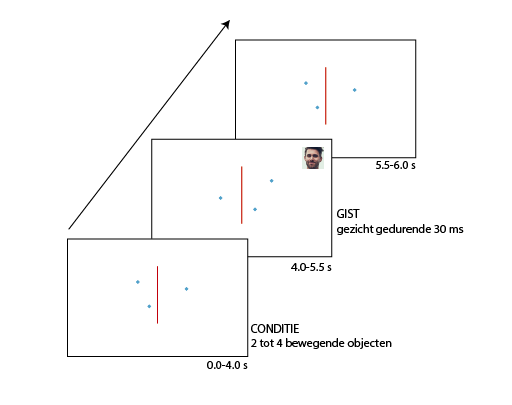
\includegraphics[width=1.0\linewidth]{Methode.png}
    \caption{\label{fig:tijdlijnExperiment}Schematische weergave van het experiment.}
\end{figure}
\subsubsection{Randomisatie}
De objecten kregen voor elke ronde een gerandomiseerde snelheid volgens vergelijking \ref{eq:sin} en \ref{eq:cos}, waarbij $\{f_{y} : f_{y}=\frac{a}{30}\}$ en $\{f_{x} : f_{x}=\frac{a}{60}\}$ met $\{a : \langle 0,\cdots,800\rangle\}$. Elk object kreeg elk frame (met $60fps$) met een waarde uit deze reeks  De snelheid is o.a. bepaald op basis van $v$, een random getal tussen 0.5 en 1.2. De richting werd bepaald door $d$, die een random waarde van 1 of -1 aannam.
\begin{align}
y = 50 \cdot sin(f_{y} \pi (\frac{v_{z} b_{i}}{2}) \label{eq:sin}
\\
x = d \cdot 150 \cdot cos(f_{x} \pi v_{z} b_{i}) \label{eq:cos}
\end{align}
Voor de verschillende condities hebben we de snelheid $v_{z} b_{i}$ voor elk object $i$ aangepast volgens tabel \ref{tab:randomSnelheden}. 
\begin{table}
\caption{\label{tab:randomSnelheden}Randomisatie snelheden objecten.}
\begin{tabular}{c c c c c}\hline
\centering
	& \underline{$b_{1}$} & \underline{$b_{2}$} & \underline{$b_{3}$} & \underline{$b_{4}$} \\
	2 objecten & 1.0 & 1.0 & NA & NA\\
	3 objecten & 0.8 & 0.8 & 0.5 & NA\\
	4 objecten & 0.8 & 0.8 & 0.7 & 0.5 \\
\hline
\end{tabular}
\end{table}
De bovengrens van $v$ voor 4 objecten is bepaald op basis van een kleine (n=6) snelheidstest. De proefpersonen beoordeelden hierbij het tellen van 4 objecten (met oplopende snelheden) en gaven aan het einde van elke ronde op een 5-punts-likertschaal \cite{likert1932technique} aan hoe goed de snelheid te hanteren was (waarbij hoe hoger de score, hoe gemakkelijker de objecten te tellen waren). Omdat voor een snelheid van 1.0 een gemiddelde beoordeling van $2.3 \pm 0.3$ werd gegeven, is dit als bovengrens genomen voor randomisatie van de conditie met 4 objecten ($v_{z} b_{1,2} = 1.2 \cdot 0.8 = 0.96$). Te hoge snelheden (die beoordeeld werden met een 1) zouden de proefpersonen namelijk kunnen laten opgeven ("dit is echt niet te doen!"), waardoor de kans zou bestaan dat ze alsnog hun focus zouden verliezen. Als dat zou gebeuren, bestond het risico dat alsnog onbedoeld oogbewegingen als contaminerende variabele werden geïntroduceerd bij de hogere snelheden. De extra variatie via $b_{i}$ hebben we aangebracht om te voorkomen dat de objecten teveel zouden groeperen. De intensiteit van het volgen van 4 objecten werd namelijk aanzienlijk eenvoudiger, wanneer de 4 objecten zich 2-aan-2 groepeerden. 
\subsubsection{Taken} De aandachtstaak van de proefpersonen was om te tellen hoe vaak de objecten de rode lijn kruisten. De bewustzijnstaak bestond uit het tegelijkertijd waarnemen van afbeeldingen met een mannen-, dan wel vrouwengezicht (zie figuur \ref{fig:tijdlijnExperiment}). 
Deze afbeeldingen (150x150 pixels) groot werden gerandomiseerd gekozen uit een set van 40 mannen- en 40 vrouwengezichten, geselecteerd op dezelfde etniciteit als onze proefpersonen (om te voorkomen dat dit een contaminerende variabele zou kunnen worden \cite{sporer2001recognizing}) getoond. De afbeeldingen werden tussen 4.0s-5.5s getoond voor 30ms, random op een y-positie van 250,0 of -250 en een x-positie van 250 of -250. Het experiment werd voor elke conditie (2, 3 of 4 objecten) 20 keer herhaald, in een volledig mixed design (zie figuur \ref{fig:mixedDesign}, waarbij elke conditie steeds \'e\'en keer werd herhaald, zodat de proefpersonen in totaal 60 rondes hadden. Er is voor een mixed design gekozen om uit te sluiten dat er een groter trainingseffect zou plaatsvinden in een van de condities. Na 6 seconden verscheen een rapportagescherm, waarbij proefpersonen voor de gistafbeelding konden kiezen uit \textquotedblright man\textquotedblright, \textquotedblright vrouw\textquotedblright\, of\, \textquotedblright geen afbeelding gezien\textquotedblright. Voor de objecten konden de proefpersonen rapporteren hoe vaak deze de rode lijn hadden gekruist. Het observeren duurde steeds 6 minuten. Het gehele experiment, inclusief het rapporteren, duurde ongeveer 10 minuten.

\subsubsection{Analyse}
De analyse is uitgevoerd met behulp van de R-software \cite{Rsoftware}. PsychoPy sloeg voor elke trial de data op in een .csv bestand, wat vervolgens wordt uitgelezen door R. Met behulp van het tidyverse-package \cite{tidyverse} is de data bewerkt en gesorteerd. Prestatie op objecttelling en gistwaarneming waren de afhankelijke variabelen, de intensiteit van de aandachtstaak (conditie 2, 3 en 4) de onafhankelijke variabele. Met behulp van het ggplot2-package \cite{ggplot} zijn op basis van deze gegevens grafische weergaven gemaakt. Van diverse (sub)sets zijn lineaire regressies gemaakt waardoor uitspraken mogelijk zijn over de resultaten in verhouding tot onze hypothese. Voor effecten van sekse, leeftijd en aandachtsstoornis is gecontroleerd.
\begin{figure}
\centering
	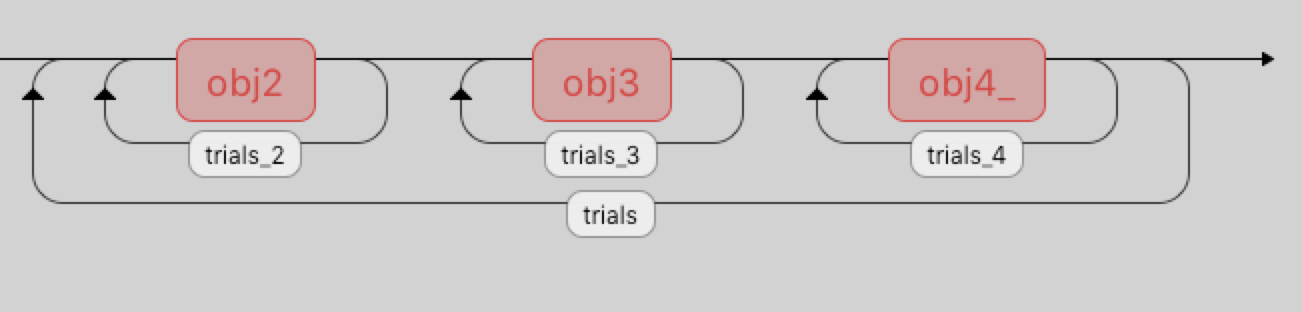
\includegraphics[width=1.0\linewidth]{opzetExperiment.png}
    \caption{\label{fig:mixedDesign}Mixed design van de condities}
\end{figure}
\section*{Resultaten}
\subsection{Toename van aandachtsintensiteit}
De hypothese gaat ervan uit dat de verschillende condities in toenemende mate de aandacht monopoliseren. Daarom is gecontroleerd of dit ook in de data zichtbaar werd en de aandachtstaken inderdaad toenamen in moeilijkheid. Een goede graadmeter hiervoor is het aantal fouten dat proefpersonen maken in het tellen van de objecten. Wanneer de spreiding van deze waarden in tabel \ref{tab:objecttelling} wordt bekeken is inderdaad zichtbaar dat de gemiddelde waarde voor conditie 2 en 3 significant hoger ligt dan de gemiddelde waarde voor conditie 4. Dit suggereert dat conditie 4 inderdaad een zwaarder beroep doet op de aandachtstaak dan bij conditie 2 en 3.
\begin{table}
\caption{\label{tab:objecttelling}Spreiding van objecttelling per conditie.}
\begin{tabular}{c c c c c}\hline
\centering
	 &  \underline{mean}  & \underline{SDM} & \underline{min} & \underline{max}\\
	conditie 2 & 91.08 & 1.17 & 70 & 100\\
	conditie 3 & 91.32 & 1.51 & 70 & 100\\
	conditie 4 & 85.98 & 1.71 & 60 & 100\\
	\hline\\
\end{tabular}
\end{table}
\begin{figure}
\centering
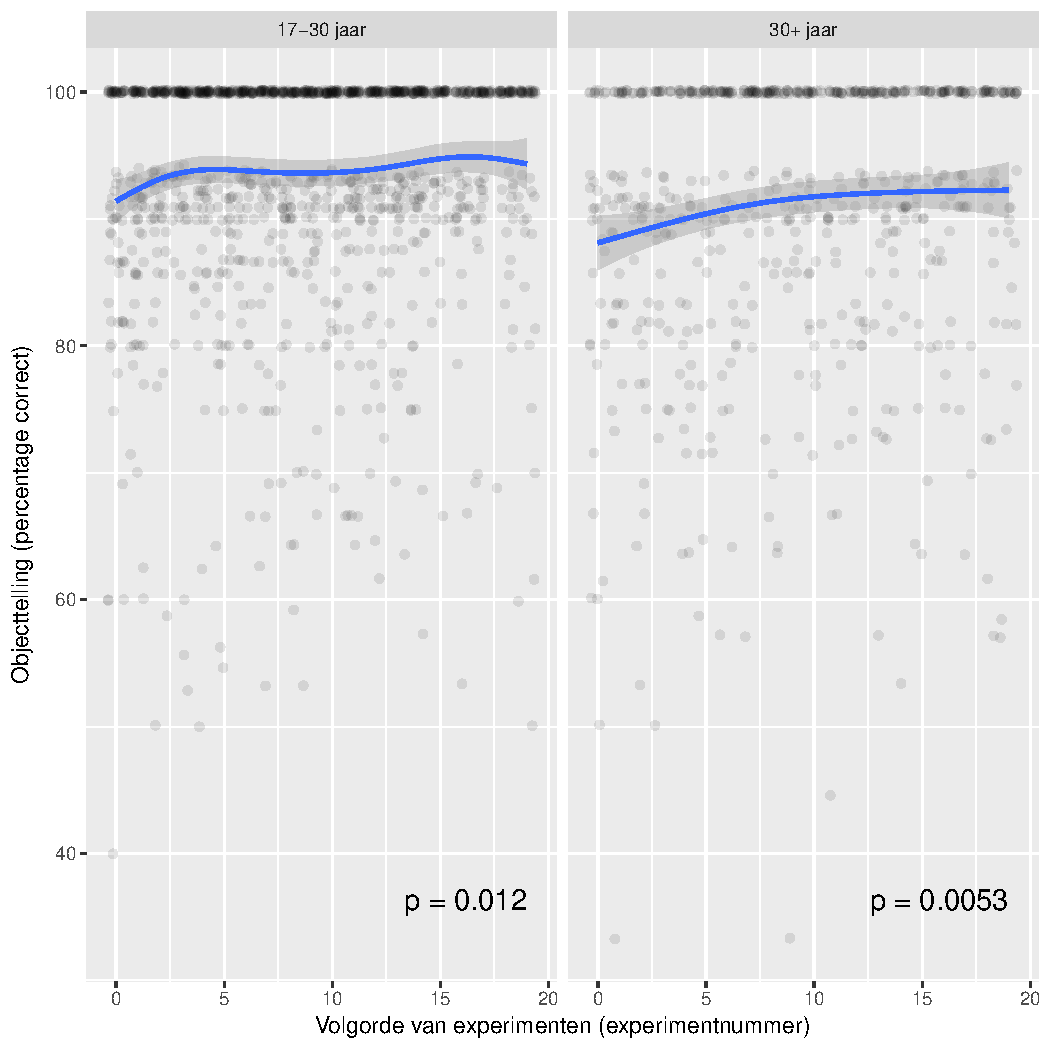
\includegraphics[width=1.0\linewidth]{training-grid.pdf}
\caption{\label{fig:objecttellingGrid}Trainings- en vermoeidheidseffect. Verloop prestatie objecttelling in de tijd, per leeftijdsgroep. De blauwe lijn is een lineaire regressie.}
\end{figure}
\subsection{Trainings- en vermoeidheidseffecten}
Omdat we een trainingseffect verwachtten, zijn er diverse lineaire regressies gemaakt van de prestatie op objecttelling, in combinatie met het tijdsverloop. De meest opvallende effecten zagen we wanneer we de proefpersonen opdeelden naar de leeftijdsgroepen 17-30 en 30+. Beide regressies hebben significante p-waarden van onder de 0.05 (p=0.012 en p=0.0053, zie ook figuur \ref{fig:objecttellingGrid}). De jongere leeftijdsgroep begint met een stijgende lijn, wat een trainingseffect impliceert. Dit was naar verwachting en de reden voor het gebruiken van een mixed design. Onverwachts was echter de afvlakking en zelfs de daling van de lijn. Bij sommige individuele proefpersonen is deze daling zeer sterk zichtbaar. Dit hangt waarschijnlijk samen met iets dat de proefpersonen ook regelmatig spontaan rapporteerden: na ongeveer 10 rondes zeiden diverse proefpersonen dat ze het experiment vermoeiend vonden worden. Onze hypothese is dat dit vermoeidheidseffect bij een aantal mensen zorgt voor een daling van de prestaties, na een initiële stijging van de prestatie door training. Voor de oudere leeftijdsgroep zet deze daling later in en is het minst aanwezig bij de groep oudere mannen. De vrouwen van 30+ presteerden overigens opvallend slechter qua vermoeidheidseffect, maar omdat in onze groep proefpersonen maar twee vrouwen van 30+ zaten zijn die lineaire regressies niet significant.
\subsection{Gistwaarneming}
Middels het maken van een boxplot wordt duideljk of de gistwaarneming inderdaad daalt of gelijk blijft bij een toenemende intensiteit van de aandachtstaak (zie figuur \ref{fig:boxplotGist}). Deze resultaten zijn eveneens zichtbaar in tabel \ref{tab:prestatieGist}). Gezien de standaarddeviatie van het gemiddelde is met zekerheid te zeggen dat de metingen voor conditie 2 en 3 significant verschillen van de metingen van conditie 4.
\begin{figure}
\centering
	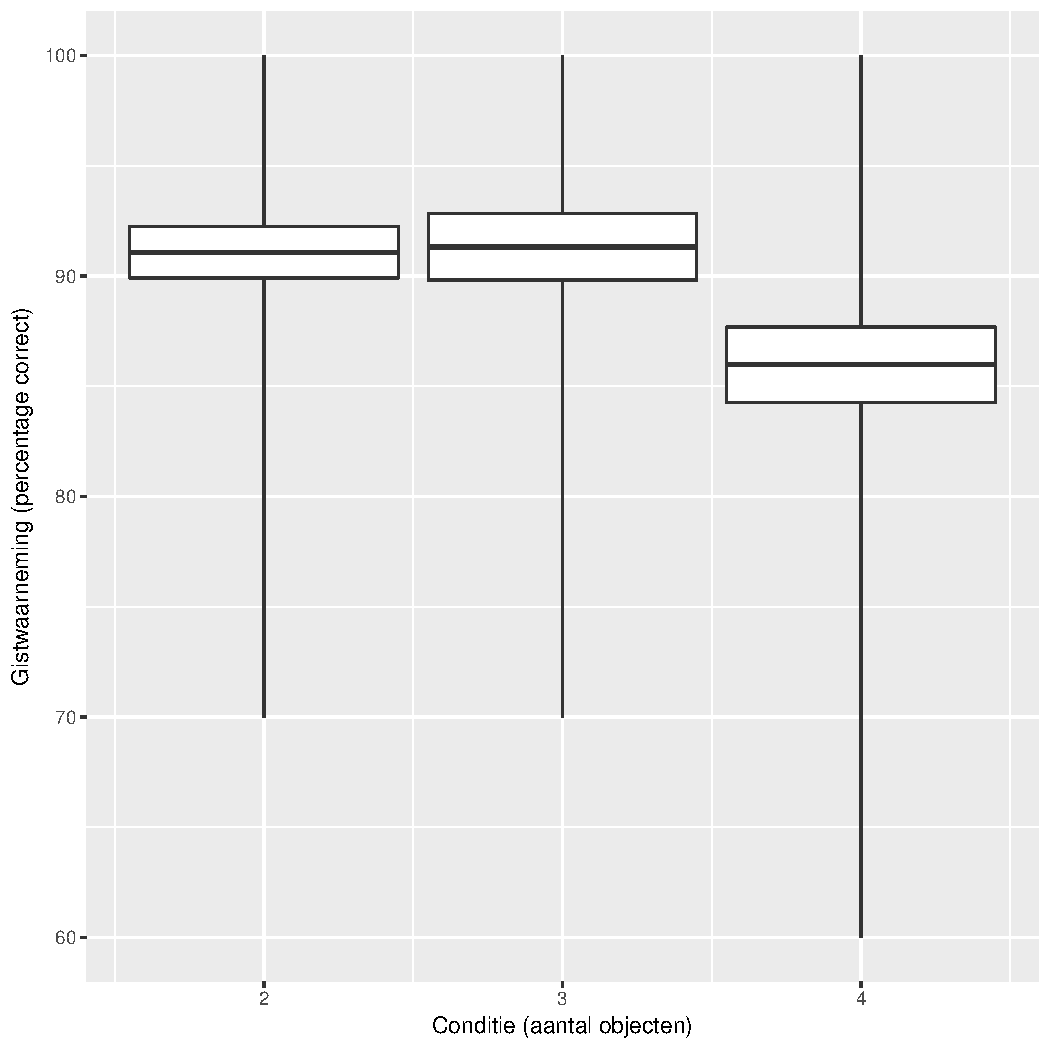
\includegraphics[width=0.8\linewidth]{boxplotGist-conditie.pdf}
	\caption{\label{fig:boxplotGist}Spreiding gistwaarneming per conditie. De errorbars geven de standaarddeviatie van het gemiddelde weer. De verticale lijn is de totale spreiding.}
\end{figure}
\begin{table}
\caption{\label{tab:prestatieGist}Prestatie gistwaarneming (in \%)}
\begin{tabular}{c c c c c}\hline
\centering
	 &  \underline{mean}  & \underline{SDM} & \underline{min} & \underline{max}\\
	conditie 2 & 91.08 & 1.17 & 70 & 100\\
	conditie 3 & 91.32 & 1.51 & 70 & 100\\
	conditie 4 & 85.98 & 1.71 & 60 & 100\\
	\hline\\
\end{tabular}
\end{table}
Wanneer we een lineaire regressie volgens de formule $f(x)=ax+b$ maken (zie figuur \ref{fig:lineaireRegressie}), zien we duidelijk dat dit een dalende lijn is. De waarde van $a=-0.025 \pm 0.01$ (t-waarde = -2.42, p-waarde = 0.017). Dit is ruim onder significantieniveau. Het percentage correcte gistwaarnemingen daalt dus wanneer de intensiteit van de aandachtstaak toeneemt. Gezien het gevonden vermoeidheidseffect hebben we gecontroleerd of het model voor verschillende afkapwaarden (waarbij alleen de eerste rondes tot en met de afkapwaarde wordt meegenomen bij modelvorming) anders zou uitvallen. In tabel \ref{tab:afkapwaarden} zijn enkele van deze waarden weergegeven. Het is duidelijk dat voor elk afkappunt de p-waarde significant blijft en $a<0$. Wel is duidelijk dat het model voor onze data het meest betrouwbaar is wanneer alleen naar de eerste 9 rondes wordt gekeken. Dit is verklaarbaar door de verschillen die er tussen proefpersonen onderling ontstaan na de 9e ronde door invloed van het vermoede vermoeidheidseffect.
 \begin{table}
 \caption{\label{tab:afkapwaarden}Invloed variatie in vermoeidheid op modelvorming.}
\begin{tabular}{c c c}
	\hline
    \centering
	\underline{p-waarde} & \underline{$a$} & \underline{afkapwaarden}\\
	0.007 & -0.035 & 9\\
	0.014 & -0.032 & 10\\
	0.043 & -0.024 & 15\\
	0.017 & -0.025 & 20\\
	\hline
\end{tabular}
 \end{table}
\begin{figure}
\centering
	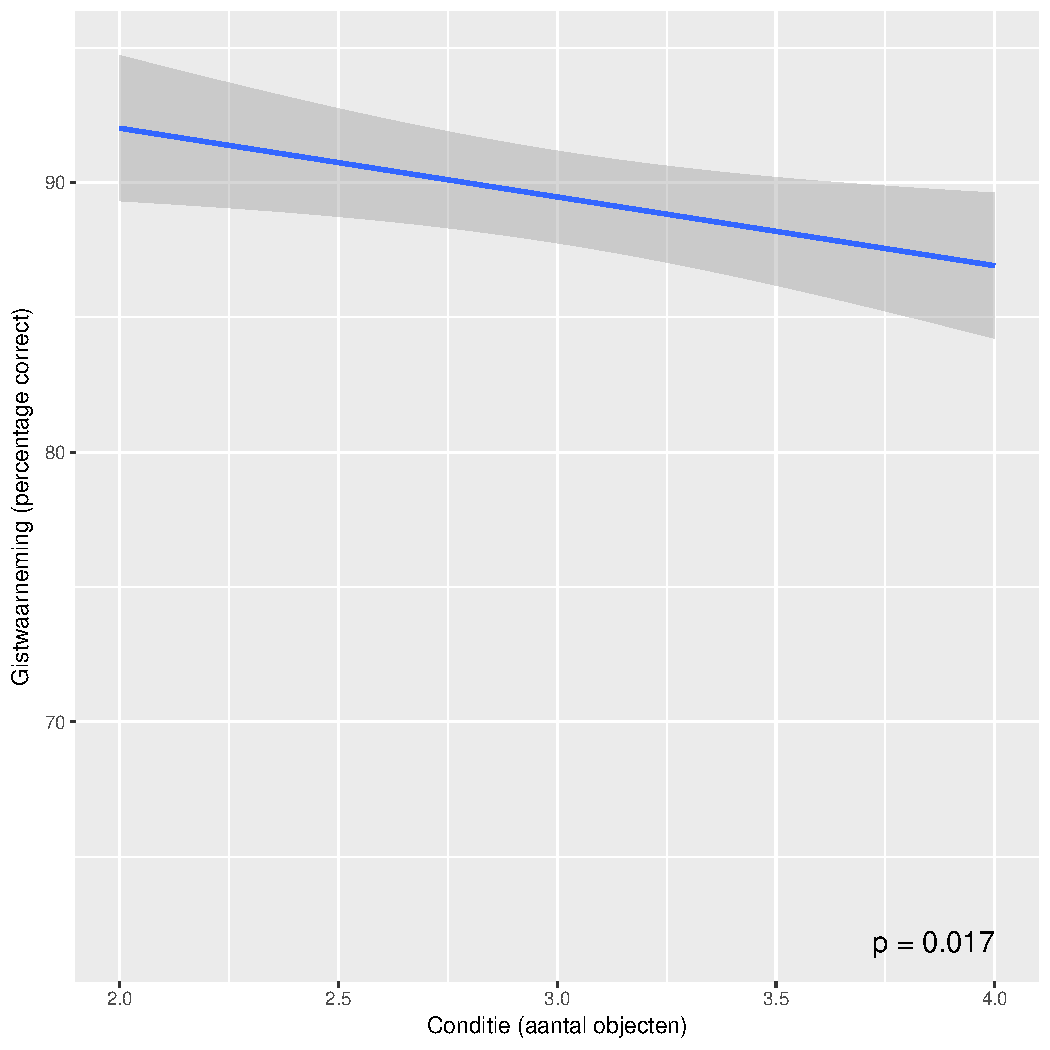
\includegraphics[width=0.8\linewidth]{lineaireRegressie.pdf}
	\caption{\label{fig:lineaireRegressie}De lineaire regressie volgens $f(x)=a x+b$ voor gistwaarneming en conditie.}
\end{figure}
\subsection*{Discussie}
Dit onderzoek betrof de vraag of bewustzijn zonder aandacht mogelijk zou zijn. Het is een complex, weerbarstig en veelzijdig onderwerp, en ook ons onderzoek geeft geen bindend antwoord is op de vraag of bewustzijn zonder aandacht bestaat. 
Omdat de kritische onderzoeken op dit gebied een aandachtsinstructie als onafhankelijke variabele bevatten, leek het van belang een onderzoek uit te voeren zonder diezelfde aandachtsinstructie met een mogelijke onbedoelde contaminatie door de daarmee ge\"introduceerde oogbewegingen. In het onderzoek van dit artikel is er juist getracht de aandacht oplopend te monopoliseren, zodat oogbewegingen zo constant mogelijk bleven. De hypothese voor dit onderzoek was dat indien aandacht een voorwaarde is voor bewustzijn, het percentage correcte gistwaarnemingen zal afnemen. Wanneer aandacht geen voorwaarde is voor bewustzijn, zullen beide taken niet interfereren en zal het percentage gistwaarnemingen niet afnemen bij een toenemende intensiteit van de aandachtstaak. Onze onderzoeksdata doet hierover meerdere significante uitspraken. Naarmate de aandachtstaak zwaarder werd (oftewel, hoe meer objecten de participant moest volgen) presteerden de participanten slechter op het tellen van de bewegende objecten. Hetzelfde gold voor de gistwaarneming. Hoe meer objecten de participanten moesten volgen met hun ogen, hoe lager het percentage correcte gistwaarneming werd. Een andere interessante uitkomst van het onderzoek is het effect waarvan wij vermoeden dat het een vermoeidheidseffect is. Er waren echter grote verschillen wat betreft dit mogelijke vermoeidheidseffect tussen bijvoorbeeld mannen en vrouwen, of tussen de oudere (30+) en de jongere leeftijdsgroep (17-30). Deze verschillen hebben invloed op de betrouwbaarheid van een lineair model omdat het monopoliseren van de aandacht na de 10e ronde tussen proefpersonen onderling sterk uiteen begon te lopen. De resultaten impliceren dat aandacht inderdaad een bijdrage levert aan bewustzijn. Dit betekent dat de stellingnamen van o.a. Block (2011) niet kan standhouden. Het betekent echter evenmin definitief dat stellingname van o.a. Cohen et al. (2012) bewezen wordt, omdat ons onderzoek niet vaststelt dat de limiet van $f(x)$ voor $x\rightarrow\inf$ gelijk is aan 0, of eenvoudigweg naar een lager niveau toe beweegt. Het probleem hierbij is dat het zeer lastig is om te bepalen wanneer werkelijk alle aandacht gemonopoliseerd wordt door de aandachtstaak. 
Een punt van verbetering voor dit onderzoek is het rekening houden met condities als ADD of ADHD bij proefpersonen. Het is nu eenmaal een aandachtsexperiment, dus het zou van belang kunnen zijn om hierop te letten, en dat is in dit geval niet gebeurd. Voor vervolgonderzoek lijkt het verder van belang de intensiteit en frequentie van de test te vari\"eren. Het viel op dat de proefpersonen vermoeid raakten na een bepaald aantal rondes van de test. Een uitslag van deze test zonder vermoeidheidseffect zou dus kunnen worden bereikt door de proefpersonen ofwel 3 keer 10 rondes te laten doen, ofwel de test op te delen in 2 maal 3 keer 10 rondes. 
\bibliographystyle{apacite}
\bibliography{biblio}
\end{document}


